\section{Introduction}
Responsable : Alain Grener, alain.grener@lip6.fr

Problématique de l'UE : synchronisation de plusieurs composants dans une architecture
multi-processeur. Exemple : accès du même périphérique par plusieurs processeurs.
Observer le moyen de communicaiton entre processeurs et l''environnement des
processeurs.
Un processeur pipeline reste synchronisé : plusieurs instructions sur le même flux
de transition. Dans le cas d'nue architecture multi-processeurs $\Rightarrow$
les unités sont nativement asynchrones, mais doivent se synchroniser.

\section{Automates d'Etats Finis Communiquants Synchrones}

Il s'agit d'un modèle mathématique, qui permet de décrire tous les systèmes
matériels numériques.
"Les états" ici est l'ensemble des valeurs intégrés à l'automate des ensembles
mémorisants. Un état est une valeur stockée dans les registres.\\

Exemple avec le processeur MIPS32 : comptons le banc de registres, PC, HI, LO, etc.
On peut comptabiliser environ 50 registres, dans ce cas le processeur MIPS32
possède $2^{50}$ états.

À chaque front montant, on met à jour l'ensemble des registres internes.
Les sorties d'un automate sont les entrées d'un autre.
Un automate porduit est l'ensemble des sous-systèmes (automates). \\


\begin{center}
  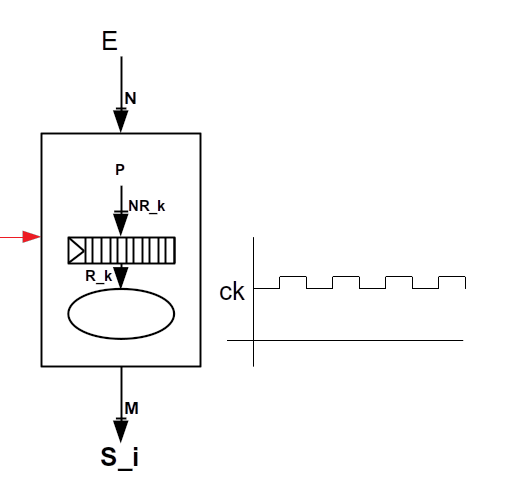
\includegraphics[height=6cm]{cours1/pics/automata.png}\\
  \(S_i=g_i(E_0,E_1,...,E_{(N-1)},R_0, R_1,...,R_{(P-1)}\), \\
  M fonctions booléennes dépendant de $N+P$ bits. \\
  \(NR_k=T_k(E_0,E_1,...,E_{(N-1)},R_0, R_1,...,R_{(P-1)}\), \\
  P fonctions booléennes dépendant de $N+P$ bits. \\
\end{center}

Pour décrire complètement le comportement d'un automate particulier, il faut déterminer:
\begin{enumerate}
  \item quelles valeurs vont prendre les sorties en fonction des entrées $E_i$ et
  de l'état. $\Rightarrow$ décrire un système séquentiel (à mémoire).
  \item les valeurs de l'état suivant $NR_k$ en fonction des entrées $E_i$ et de
  l'état courant $R_k$.
  \item un mécanisme permettant d'initialiser l'état interne $\Rightarrow$ état
  initial $R_k^{0}$.
\end{enumerate}

\subsection{Automates de Mealy vs Automates de Moore}
\begin{center}
  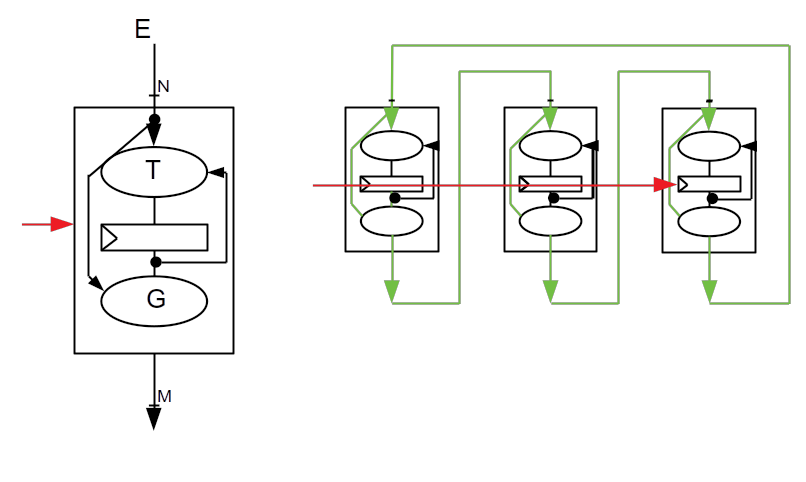
\includegraphics[height=6cm]{cours1/pics/mealy.png}
  \\La géneration de la sortie dépend de l'état de transition et des entrées
\end{center}

\begin{center}
  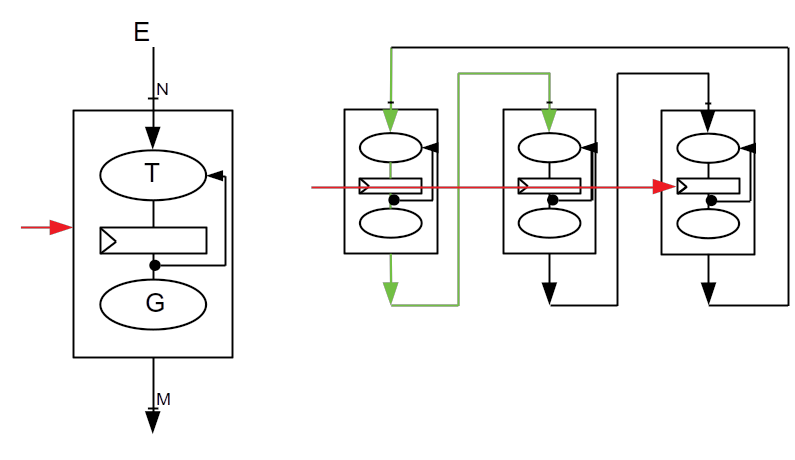
\includegraphics[height=6cm]{cours1/pics/moore.png}
  \\ La géneration de la sortie dépend uniquement de l'état de transition
\end{center}
Avantages de l'Automate de Moore :
\begin{itemize}
  \item Facilement prédictible (synchronisation assurée)
  \item Beaucoup plus stable sur la propagation de l'information
\end{itemize}
Inconvénients :
\begin{itemize}
  \item Moins réactif
\end{itemize}
Le plus long chemin possible est le temps de cycle minimal d'un registre à un
autre.
\begin{center}
  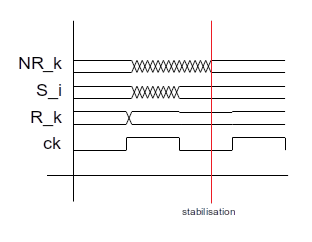
\includegraphics[height=10cm]{cours1/pics/chrono.png}
  \\ La géneration de la sortie dépend uniquement de l'état de transition
\end{center}

\section{Méthode Génerale de Synthèse des FSM}
Toute l'industrie de la CAO repose sur la technologie des FSM. \\
$\Rightarrow$ Par extension, toute l'industrie du High-Tech.

{\bf ETAPE A:}\\
Définition des "états abstraits".
Il s'agit d'identifier les états avec des symboles et faire abstraction de leur
description pour leur nomination.

{\bf ETAPE B:}\\
Représentation abstraite du graphe de transition.\\
Il va s'agir d'un graphe orienté dont on doit précisément spécifier :
\begin{itemize}
  \item Les états (un noeud par état accessible)
  \item Les transitions (les arcs orientés) :
  \begin{center}
    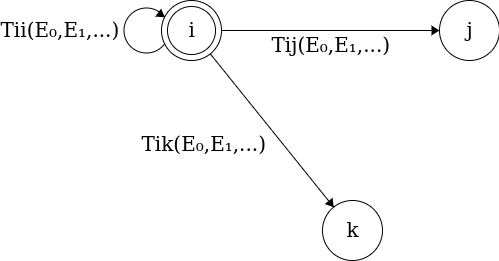
\includegraphics[height=4cm]{cours1/pics/graph1.png}
    \\On doit s'assurer des conditions d'orthogonalité et de complétude :
    \begin{itemize}
      \item orthogonalité $\Rightarrow$ 2 transitions de sortie ne peuvent pas
      être simultanément accessibles :\\
      \begin{center}
        \(\forall E_i \forall i \forall j \forall k{(T_{ij} \bullet T_{ik})} \equiv 0\) si
        $i \ne j$
      \end{center}
      \item complétude $\Rightarrow$ Il y a toujours une transition de sortie
      qui est vraie : \\
      \begin{center}
        \(\forall E_i \forall i \sum{j=0}{(T_{ij})} = 1\)
      \end{center}
      Nb : Les états sont étiquetés en fonction de fonction booléenne de l'expression
      de la valeur de sortie
    \end{itemize}
  \end{center}
\end{itemize}

{\bf ETAPE C:}\\
Choix d'un codage des états.

{\bf ETAPE D:}\\
Traduction du graphe en table de vérité.

{\bf ETAPE E:}\\
Déterminer les équations booléennes simplifiées.

{\bf ETAPE F:}\\
Traduction en portes logiques

\subsection{Exemple : capteur de trois '1' consécutifs, MOORE}

Etape A :
\begin{itemize}
  \item "ZERO", aucun chiffre mémorisé
  \item "UN", le dernier caractère detecté est 1
  \item "DEUX", les deux derniers caractères détectés sont '1' et '1'
  \item "TROIS", les trois derniers caractères détectés sont '1','1' et '1'
\end{itemize}

Etape B :\\
\begin{center}
  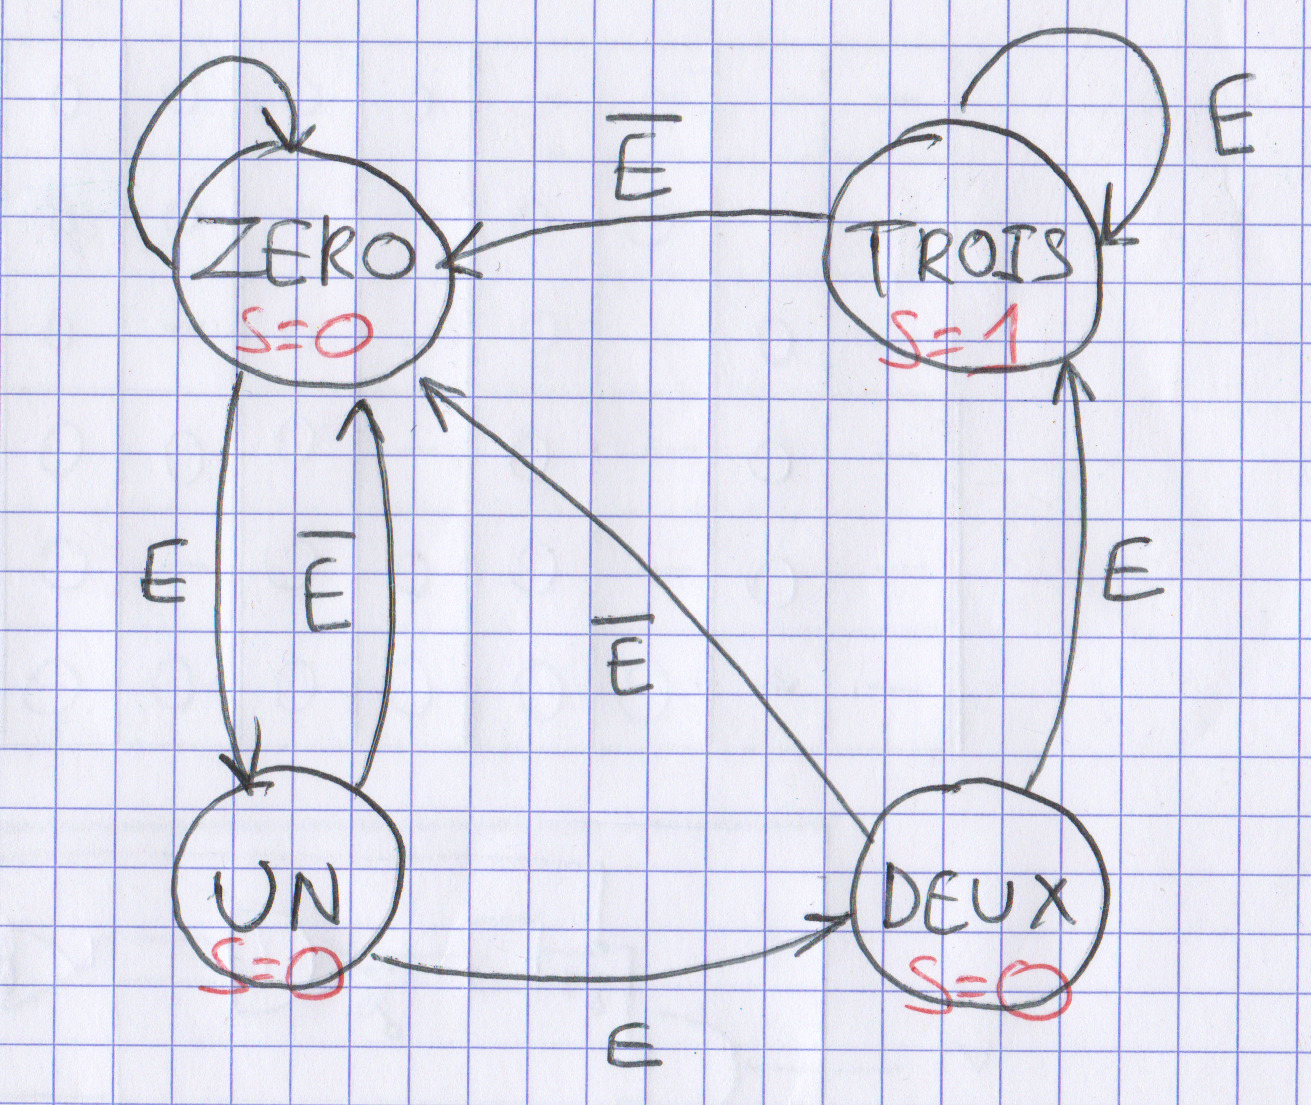
\includegraphics[height=6cm]{cours1/pics/graph2.png}
\end{center}

Etape C :
\begin{center}
  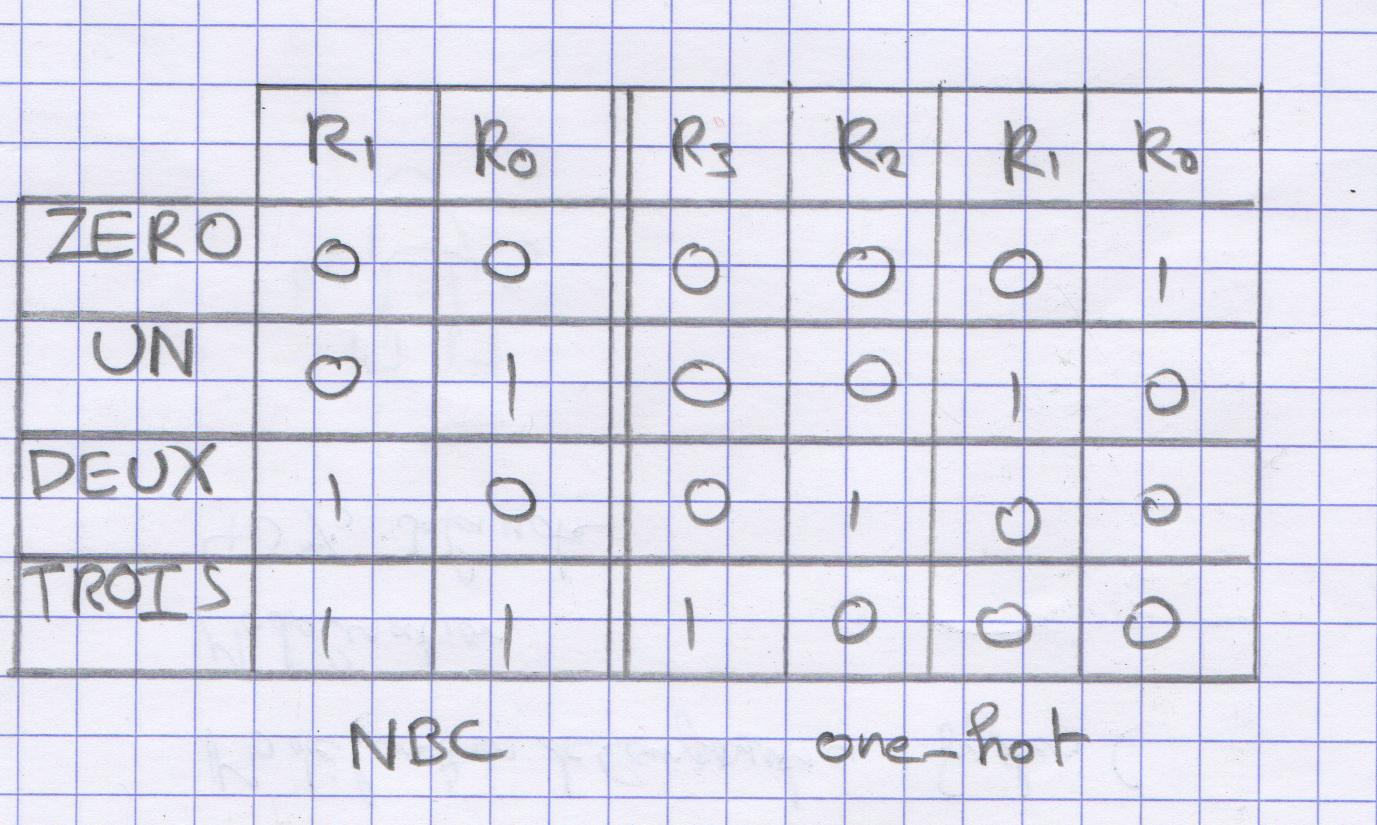
\includegraphics[height=6cm]{cours1/pics/truthtable.png}
\end{center}

Etape D
\begin{center}
  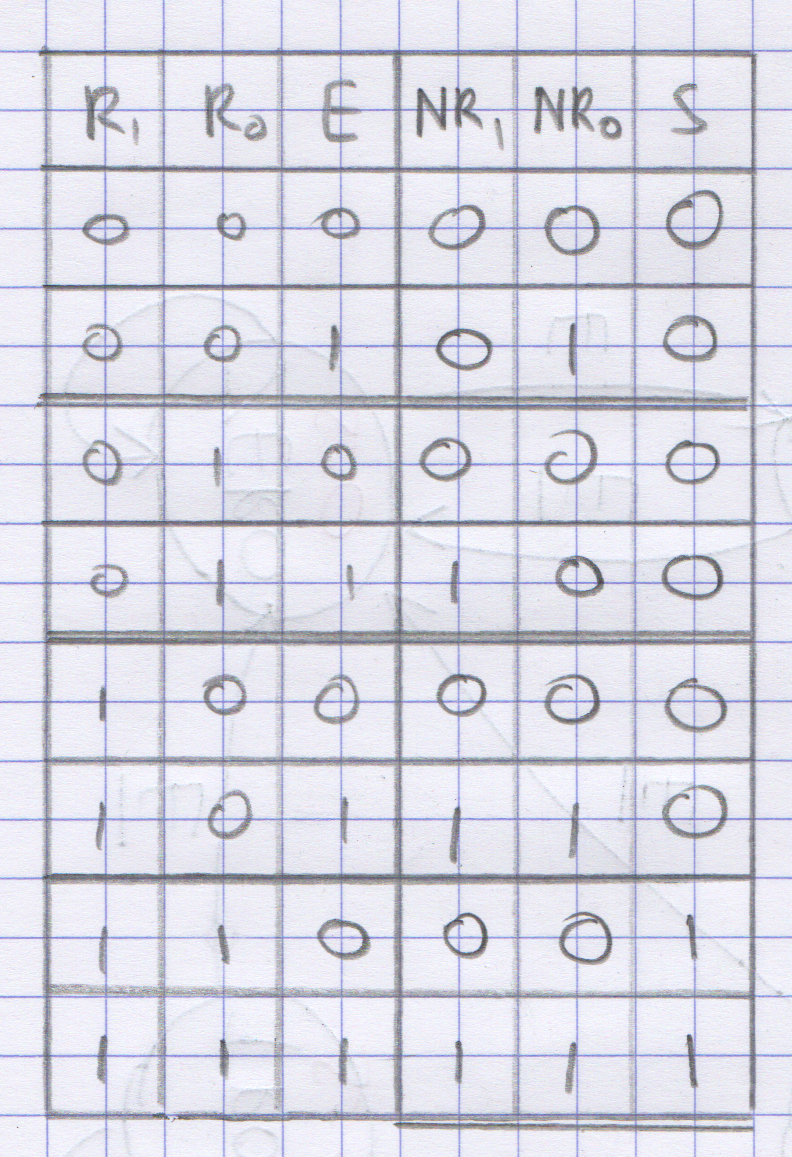
\includegraphics[height=6cm]{cours1/pics/equationtable.png}
\end{center}

Etape E
\begin{itemize}
  \item \(S=R_1 \bullet R_0\)
  \item \(NR_1 = E \bullet {(R_0 + R_1)}\)
  \item \(NR_1 = E \bullet {(\overline{R_0} + R_1)}\)
\end{itemize}

Etape F
\begin{center}
  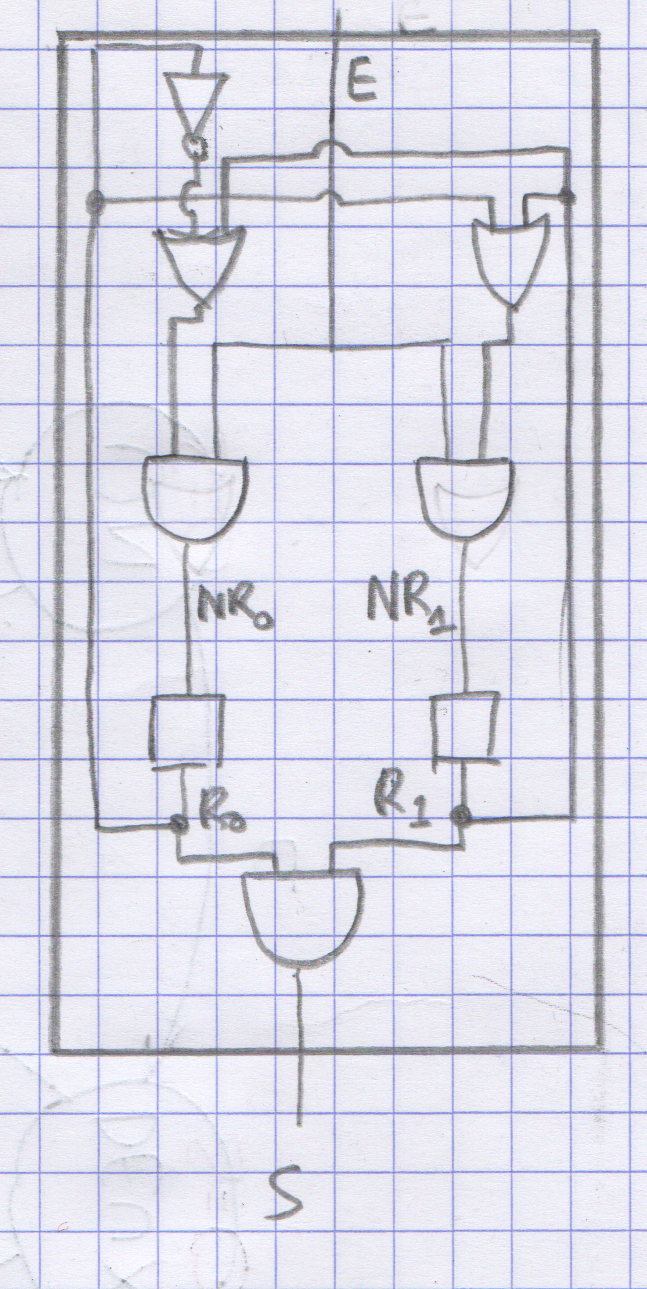
\includegraphics[height=6cm]{cours1/pics/circuit.png}
\end{center}
